% !TeX root = ../main.tex

\chapter{系统需求分析及架构设计}
本章节系统全面介绍了视频表决会议系统的需求分析及架构设计工作。本章节从系统业务出发,分析了视频表决会议系统的需求,根据需求进行了针对性的架构设计,并介绍了与原会议系统的区别之处。

\section{需求分析}

会议系统根据功能性质划分,分为两个大的模块,一是会议管理模块,另一个是会议系统主模块。运营平台会议管理模块负责会议的创建、修改及数据导入等会议管理功能。会议系统主模块负责视频直播、投票表决、实时查看数据、实时聊天等会议核心功能。

\subsection{会议管理模块}

会议系统管理模块负责会议管理相关的功能,会议的管理模块由运营人员在运营平台进行操作,运营人员具有的功能权限有创建/修改会议、导入表决数据、导入其他参会人员信息、获取密码反馈、激活会议、发送短信通知及获取推流地址。会议系统管理模块的具体功能需求如图~\ref{fig:meetingManagement} 所示。

\begin{figure}[!htp]
  \centering
  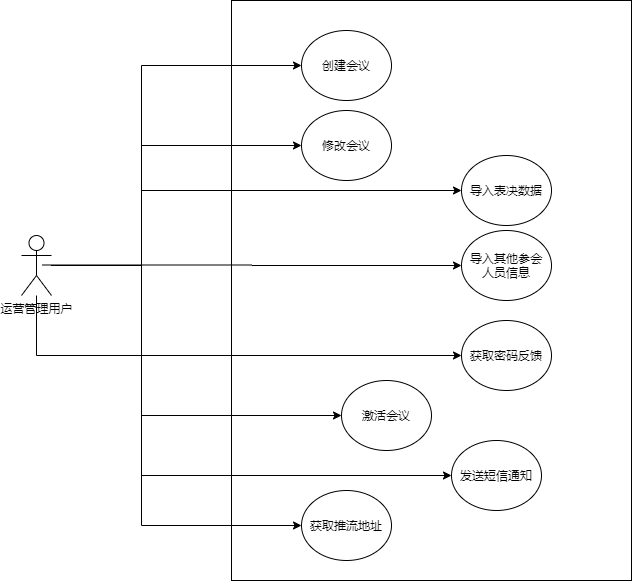
\includegraphics[height=10cm]{meetingManagement.png}
  \caption[管理模块]
    {会议系统管理模块需求用例图}
 \label{fig:meetingManagement}
\end{figure}

\subsubsection{创建和修改会议}
原系统会议模块创建和修改会议分为三步,填写会议基本信息、填写议题相关信息、导入议题表决信息。导入议题表决信息显然和创建会议属于不同功能,将导入信息作为创建会议的一环并不合理,因此将导入议题表决信息功能单独拆出。另外将创建会议拆分成两步并没有实际意义,反而增加了创建会议时出现错误的概率,因此将填写会议基本信息、填写议题相关信息合并为一步。

运营管理人员在运营平台创建和修改会议。创建和修改会议需要填写会议的基本信息(会议名称和会议召开日期为必填项)、会议的议程信息(包括需表决和无需表决议程)、议程的表决组信息,由于向 OSS 文件系统存储会议文件和议程文件时,需要会议号作为索引,因此在创建会议前需要提前向后端请求获取预约会议号。

\subsubsection{导入表决数据和其他参会人员信息}
表决数据包括表决信息(表决所在表决组、表决金额等)和表决信息对应的债权人信息。原系统会议模块导入表决数据是创建会议的第三步,表决数据仅可导入原债权申报系统中已存在的数据,若仅使用会议功能,表决数据的导入和原债权申报系统数据强绑定的设计就显得极为不合理。因此将导入表决数据和原债权申报系统数据解除绑定,改为使用 Excel 文件上传导入表决数据。点击下载 Excel 模板,填写完表决数据完整信息后,点击导入表决数据上传填好的 Excel 文件。此时,可能存在债权人未在会议平台注册的情况,表决数据若对应已存在债权人,则将表决数据划分给已存在债权人。表决数据若对应不存在债权人,则先创建对应债权人,再将表决数据划给创建的债权人。

会议除相关管理人和债权人外,还存在其他参会人员(仅可观看会议)。其他参会人员不可自行注册,仅可通过运营人员在运营平台通过上传 Excel 文件导入,目的是为了防止会议无关人员参与会议。

\subsubsection{发送短信通知}
与原系统会议模块相比,增加了短信通知功能。运营平台管理员可以向所有会议相关人员发送短信通知。选定模板和发送范围后,可以向指定范围发送会议相关信息。

\subsection{会议系统主模块}

原系统会议模块用户分为两类。一是管理人用户,二是债权人用户。若存在仅可观看会议的其他类型参会人员,需注册为债权人用户,不赋予表决数据,即可满足只能观看的需求。这种做法不符合规范,因此新增游客用户类型,仅提供观看会议的权限。

会议系统主模块负责会议的核心功能。视频表决会议系统的用户分为三类。一是管理人用户,二是债权人用户,三是游客用户(即其他参会人员)。管理人用户具有开启表决、结束表决、查看表决详情、查看参会详情、设定结束日期、查看会议详情、查看会议列表、观看视频直播、实时聊天的功能。债权人用户具有签到、补签、投票表决、实时聊天、查看会议列表、查看会议详情、观看视频直播的功能。游客用户具有查看会议列表、查看会议详情、观看视频直播的功能。会议系统主模块的具体功能需求如图~\ref{fig:meetingMain} 所示。

会议系统主模块功能根据是否有实时性要求又分为实时模块和非实时模块。实时模块包括实时聊天功能和投票表决功能。

\begin{figure}[!htp]
  \centering
  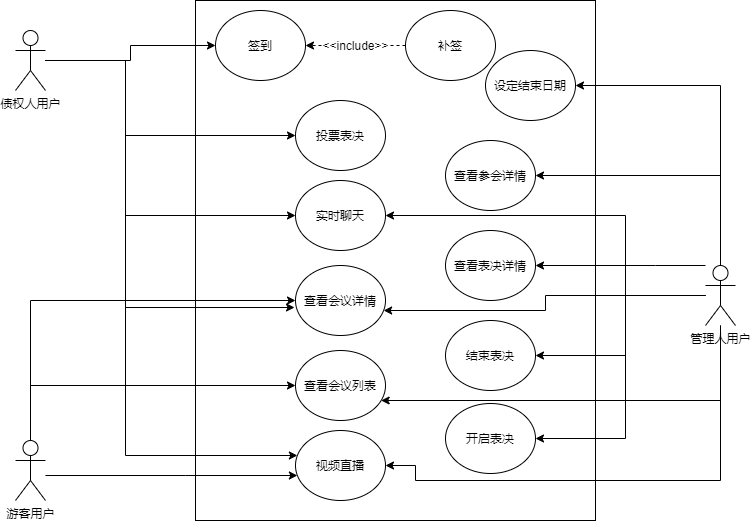
\includegraphics[width=12cm]{meetingMain.png}
  \caption[主模块]
    {会议系统主模块需求用例图}
 \label{fig:meetingMain}
\end{figure}

\subsubsection{开启和结束表决}
原系统会议模块的表决开启和结束由创建会议时设定的开启日期和结束日期决定,由于实际需求中,会议的表决开启和结束有时需要管理人进行控制,因此管理人用户增加了开启和结束表决的功能。

\subsubsection{查看参会详情和表决详情}
原系统会议模块仅有参看表决详情功能。在实际的会议中,管理人有时需要向法院报告会议参会情况,因此管理人用户增加了查看表决详情的功能。

\subsubsection{签到和补签}
原系统会议模块中,债权人参加会议功能在任何时间都可以使用,即时会议已经结束,债权人仍可点击参会,这与常理不符。现在改为债权人在会议开始到会议结束之间第一次进入会议时,会主动弹出签到框,提醒债权人签到参会,并提供补签功能,签到成功后才可进行投票表决。

\section{架构设计}
在破产领域中,债权人会议和表决的意义十分重大,决定着一个破产项目的走向。在一次实际的债权人会议中,债权人的数量级平均为千人级别,有些会议的债权人数量甚至可以达到上万人。债权人会议的一项重要工作是进行表决。在实际的会议中,表决可能在较短的时间内进行,因此会导致在短时间内出现大量请求。当同时有多个会议进行时,短时间激增的请求会给服务器带来极大的压力,因此需要针对性的设计架构应对此问题。

\subsection{现有架构及问题}

\subsubsection{现有架构}
\begin{figure}[!htp]
  \centering
  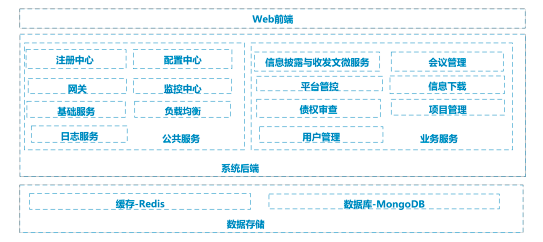
\includegraphics[width=12cm]{oldMeeting_1.png}
  \caption[原微服务]
    {原系统微服务架构图\cite{Wang2021}}
 \label{fig:oldMeeting_1}
\end{figure}

原系统采用微服务架构的原因一是原系统已具有比较完整
的服务治理管理体系,采用微服务架构将节省部署运维和降低系统升级的工作难度。这样
就能充分复用原系统的实现,减少开发系统,升级系统的成本。二是可以满足系统可
扩展性的要求。当需要对系统持续升级与优化时,可以直接设计其他微服务加入到微
服务治理体系中以满足用户不断扩展的需求。具体架构如图~\ref{fig:oldMeeting_1}\cite{Wang2021} 所示。根据微服务架构设计的高内聚低耦合的原则,原系统将会议管理整体划分为一个微服务,所有会议相关的功能全部集中放在会议管理微服务中。

在原系统的设计中,当用户数上升时,可以为各个微服
务起多个实例同时服务来满足用户并发数,可以在不改变软件架构的基础上通
过增加硬件资源来提高服务质量。

原系统是在 k8s 集群上进行部署的,系统采用图~\ref{fig:oldMeeting_2}
的物理架构。系统用户可以直接通过浏览器访问系统。而用户的请求都将到达 K8s 集群中
的 Mater Node,由 Master Node 结点进行处理。Mater Node 结点是整个集群的管理结点,该
结点会根据请求的特性命令 Work Node 结点进行作业工作。另外,一个服务往往运行成多个实例以增加系统的容错性。

\begin{figure}[!htp]
  \centering
  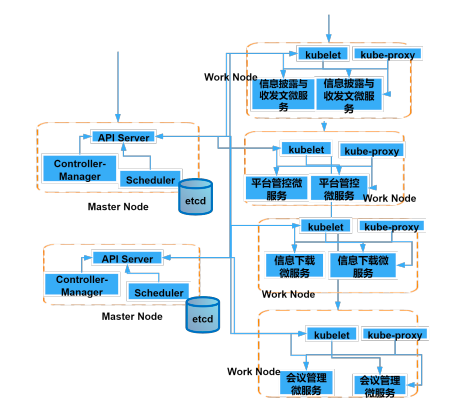
\includegraphics[height=6cm]{oldMeeting_2.png}
  \caption[原物理架构]
    {原系统物理架构图\cite{Wang2021}}
 \label{fig:oldMeeting_2}
\end{figure}

\nocite{Wang2021}
\subsubsection{存在问题}

在网络债权人会议中,保证实时性非常重要。在原系统的实现中,会议管理微服务实现为 SpringBoot 后端,在会议管理微服务中通过 WebSocket 实现实时聊天,通过轮询实现管理人查询数据的实时更新。

首先,假设系统需要能同时处理 1 万场会议,每个会议债权人数量为 1万人,仅仅实时聊天的长链接数量就达到了1亿级别。SpringBoot 项目的默认启动容器是 Tomcat,而 Tomcat 默认支持的连接数量为 1 万,这个数量级远远低于要求。如果将 WebSocket 实现在 SpringBoot 项目中,需要调大 Tomcat 的连接数量或者更换启动容器,即使更换启动容器将连接数量扩大至百万级,按照原系统设计为会议管理微服务起多个实例同时服务来满足并发数需要启动接近1百个实例,这仅仅是为了满足保持实时聊天的长连接数量。

其次,通过轮询方式实现管理人端查看数据的实时更新,会给服务器带来较大的压力,且比较浪费资源,债权人侧投票表决和管理人侧数据实时刷新也应当通过 WebScoket 实现。

我们发现在会议系统中,需要通过 WebScoket 实现的功能和其余功能是独立的,并且在现有设计下为了保证 WebScoket 的长连接数量会给服务器带极大压力和资源浪费,因此考虑将 WebSocket 相关功能拆出实现为独立的微服务。

\subsection{架构设计}
将原本的会议管理微服务拆分为会议管理微服务(除去实时功能)、实时表决微服务和实时聊天微服务。新的会议管理微服务仅包含基础功能(创建会议等),与原本实现差别不大。会议开始前和会议结束后的表决数据查询通过会议管理微服务,而在会议进行中时,表决数据查询通过实时微服务进行,后面主要介绍实时微服务架构设计。

针对系统的某个实时微服务,如表决服务、聊天服务,所有用户均使用同一套服务架构。
该服务架构一定包括无状态的 WebSocket 实例(后文简称 “实例”),以及独立的有状态 Redis 服务。Redis 服务是实例的状态中心,存储实例的所有状态数据。
采用分布式集群方案,服务架构如图~\ref{fig:cluster}。

\begin{figure}[!htp]
  \centering
  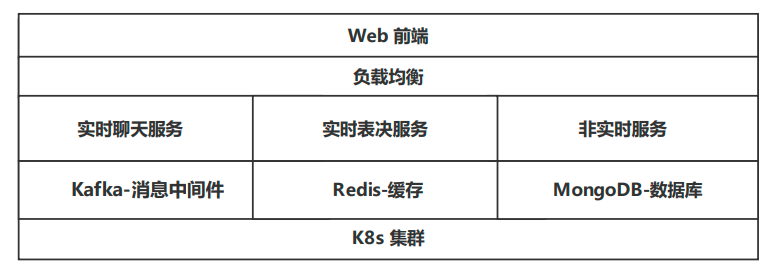
\includegraphics[width=12cm]{cluster.png}
  \caption[实时微服务架构]
    {实时微服务架构图}
 \label{fig:cluster}
\end{figure}
